% Template for NIME 2023

% Modified by Adnan Marquez-Borbon 30 November 2022
% Modified by Courtney Reed 28 November 2022
% Modified by Joe Wright 14 December 2019
% Modified by Niccolò Granieri 10 October 2018 
% Modified by Angelo Fraietta 23 December 2018
% Modified by Angelo Fraietta 22 November 2018
% Modified by Rodrigo Schramm on 22 September 2018
% Modified by Luke Dahl on 17 October 2-17
% Modified by Cumhur Erkut on <2016-10-11 Tue>
% Modified by Edgar Berdahl on 5 November 2014
% Modified by Baptiste Caramiaux on 25 November 2013
% Modified by Kyogu Lee on 7 October 2012
% Modified by Georg Essl on 7 November 2011
%
% Based on "sig-alternate.tex" V1.9 April 2009
% This file should be compiled with "nime-alternate.cls"

\documentclass{nime-alternate} % Uncomment when publishing final version

% Uncomment only one of the ones below
\usepackage{anonymize} 		   %Uncomment this line to publish
% \usepackage[blind]{anonymize}%Uncomment this line for blind review

% Package that enables the use of accents and non 
% standard characters
\usepackage[utf8]{inputenc}

\begin{document}

% --- Author Metadata here ---
%\conferenceinfo{NIME'17,}{May 15-19, 2017, Aalborg University Copenhagen, Denmark.}
%\conferenceinfo{NIME'18,}{June 3-6, 2018, Blacksburg, Virginia, USA.}
%\conferenceinfo{NIME'19,}{June 3-6, 2019, Federal University of Rio Grande do Sul, ~~~~~~  Porto Alegre,  Brazil.}
% \conferenceinfo{NIME'20,}{July 21-25, 2020, Royal Birmingham Conservatoire, ~~~~~~~~~~~~ Birmingham City University, Birmingham, United Kingdom.}
%\conferenceinfo{NIME'22,}{June 28 - July 1, 2022, Waipapa Taumata Rau, T\={a}maki ~~~~~~~~ Makaurau, Aotearoa}

\conferenceinfo{NIME'24,}{4--6 September, Utrecht, The Netherlands.}

\title{Computational analysis of guitar vibrato for extended guitar techniques}

% You need the command \numberofauthors to handle the 'placement
% and alignment' of the authors beneath the title.
%
% For aesthetic reasons, we recommend 'three authors at a time'
% i.e. three 'name/affiliation blocks' be placed beneath the title.
%
% NOTE: You are NOT restricted in how many 'rows' of
% "name/affiliations" may appear. We just ask that you restrict
% the number of 'columns' to three.
%
% Because of the available 'opening page real-estate'
\label{key}% we ask you to refrain from putting more than six authors
% (two rows with three columns) beneath the article title.
% More than six makes the first-page appear very cluttered indeed.
%
% Use the \alignauthor commands to handle the names
% and affiliations for an 'aesthetic maximum' of six authors.
% Add names, affiliations, addresses for
% the seventh etc. author(s) as the argument for the
% \additionalauthors command.
% These 'additional authors' will be output/set for you
% without further effort on your part as the last section in
% the body of your article BEFORE References or any Appendices.

\numberofauthors{1} %  in this sample file, there are a *total*
% of EIGHT authors. SIX appear on the 'first-page' (for formatting
% reasons) and the remaining two appear in the \additionalauthors section.
%
\author{
% You can go ahead and credit any number of authors here,
% e.g. one 'row of three' or two rows (consisting of one row of three
% and a second row of one, two or three).
%
% The command \alignauthor (no curly braces needed) should
% precede each author name, affiliation/snail-mail address and
% e-mail address. Additionally, tag each line of
% affiliation/address with \affaddr, and tag the
% e-mail address with \email.
%
% 1st. author
\alignauthor
\anonymize{Ben Trovato}\\
       \affaddr{\anonymize{Institute for Clarity in Documentation}}\\
       \affaddr{\anonymize{1932 Wallamaloo Lane}}\\
       \affaddr{\anonymize{Wallamaloo, New Zealand}}\\
       \email{\anonymize{trovato@corporation.com}}
% 2nd. author
\alignauthor
\anonymize{G.K.M. Tobin}\\
       \affaddr{\anonymize{Institute for Clarity in Documentation}}\\
       \affaddr{\anonymize{P.O. Box 1212}}\\
       \affaddr{\anonymize{Dublin, Ohio 43017-6221}}\\
       \email{\anonymize{webmaster@marysville-ohio.com}}
% 3rd. author
\alignauthor \anonymize{Lars Th{\o}rv{\"a}ld}\\
       \affaddr{\anonymize{The Th{\o}rv{\"a}ld Group}}\\
       \affaddr{\anonymize{1 Th{\o}rv{\"a}ld Circle}}\\
       \affaddr{\anonymize{Hekla, Iceland}}\\
       \email{l\anonymize{arst@affiliation.org}}
}
% There's nothing stopping you putting the seventh, eighth, etc.
% author on the opening page (as the 'third row') but we ask,
% for aesthetic reasons that you place these 'additional authors'
% in the \additional authors block, viz.
\additionalauthors{Additional authors: \anonymize{John Smith (The Th{\o}rv{\"a}ld Group,}
email: {\texttt{\anonymize{jsmith@affiliation.org}}}) and \anonymize{Julius P.~Kumquat 
(K. Consortium,} email: {\texttt{\anonymize{jpkumquat@consortium.net}}}).}
\date{30 July 1999}
% Just remember to make sure that the TOTAL number of authors
% is the number that will appear on the first page PLUS the
% number that will appear in the \additionalauthors section.

% For your initial submission you MUST ANONYMIZE the authors.

\maketitle

\begin{abstract}



\end{abstract} 
%\keywords{Autonomous Agents, Interactive Music System, Improvisation}

% ------- CCS Concepts
% Here is where you enter the CCS Concepts for your paper.
%
% It is strongly recommended that authors view the submission form
% prior to starting to write the paper, which includes information 
% on the CCS Concepts. 
% 
% The 2012 ACM Computing Classification System (CCS) replaces the
% traditional 1998 version, which has served as the de facto 
% standard classification system for the computing field. It is
% being integrated into the search capabilities and visual topic 
% displays of the ACM Digital Library. Please enter the CCS XML code 
% for the classification terms that describe your paper. To get the 
% XML code, please use the following procedure, which is
% demonstrated using three NIME-related example terms: Applied
% computing~Sound and music computing, Applied computing~Performing
% arts, and Information systems~Music retrieval.
%
% 1) Browse to the website http://dl.acm.org/ccs_flat.cfm.
% 2) Select one to three classification terms from the website that
%    describe your paper (e.g. for the example paper Applied
%    computing~Sound and music computing, Applied 
%    computing~Performing arts, and Information systems~Music
%    retrieval.).
% 3) For each classification you need to select the relevance
%    (e.g. for this example, Sound and music computing is "high",
%    Performing arts is "low", and Music retrieval is "Medium")
% 4) Once you have selected the last term, click on "view CCS Tex
%    Code". This will generate some code, which includes some CCSXML
%    and some lines beginning with \ccsdesc.
% 5) Keep all of this code, as you will need it for entering into
%    the Precision Conference System paper submission form.
% 6) For this document, keep only the \ccsdesc lines. Here is what
%    you would paste for the classification example:

%\ccsdesc[500]{Applied computing~Sound and music computing}
%\ccsdesc[100]{Applied computing~Performing arts}
%\ccsdesc[300]{Information systems~Music retrieval}

% this line creates the CCS Concepts section.
\printccsdesc


\section{Introduction}
Electric guitar offers several ways of shaping and articulating sound: techniques such as vibrato, slide, bending, tapping modify the dynamics and the timbral characteristics of a note. The guitarist's "touch" is considered to be very personal, and the style of a guitar player largely depends on how they articulate notes. Guitar articulations are correlated to hand motion.

Recent advancements in sensing technologies have brought attention to the embodied dimensions of musical practice, and several studies have employed computational methods for analysis of embodied knowledge of specific instrumental techniques \cite{article, inbook, Schyff}. At the same time, designers of Interactive Music Systems are using real-time body sensing to integrate embodied perspectives in their digital performance systems \cite{jensenius_gestures_2021, miranda_interactive_2021}. In this context, mapping sensor data to synthesis parameters is a non trivial task, which is affected by aesthetic choices as well as by technical and perceptive constraints \cite{strauss_extensible_2023, van_nort_mapping_2014}.

My project has the objective of informing sensor mapping strategies with a computational analysis of embodied data and audio of a specific musical technique: guitar vibrato. The purpose of my project is to track hand movement of a guitar player to develop an interface for electronically-extended guitar techniques. The interface combines sound features and hand motion data to detect the kind of guitar vibrato from real-time hand movements and exposes mapping parameters for dynamic sound shaping.



\section{Background}
\subsection{Embodiment and musical gestures}
\subsection{Interactive Music Systems}
\subsection{Computational studies of instrumental techniques}


\section{System Design}

\subsection{Data Collection}
Collecting a dataset of guitar vibrato techinques mapped to the related hand movements using motion capture. For each note on the guitar, four instances will be recorded: no vibrato, vertical vibrato, horizontal vibrato and circular vibrato. For each of these, multiple recordings will be realized with different vibrato intensity. The hand movements will be recorded using the AX6 6-axis logging accelerometer and gyroscope. At the same time, audio from the guitar will be recorded using a digital audio interface. The data recording process will be repeated multiple times in order to identify the position of the sensor on the hands which guarantees the cleanest data.

\subsection{Data Preprocessing}
Segmentation and feature extraction
Are there differences in spectral shape descriptors between the different kinds of vibrato?

\subsubsection{Segmentation}

The data from audio and sensors will be aligned and each note will be segmented using transient detection. Spectral audio descriptors will be computed from each instance: loudness (dB), true-peak descriptor (dB), loudness (linear “RMS”), spectral centroid (Hz), spectral spread (Hz), spectral flatness (dB), and 6 Mfcc descriptors. The most significant features contributing to distinguishing the different kinds of vibrato will be identified using feature importance and autocorrelation coefficients.

\begin{figure}[htbp]
	\centering
		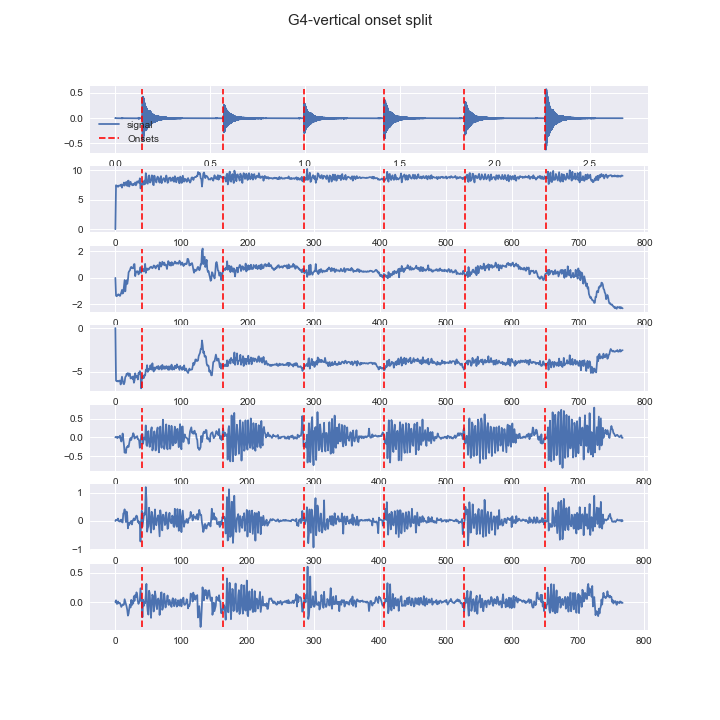
\includegraphics[width=1\columnwidth]{imgs/split.png}
	\caption{Segmentation of sound and sensor data.}
	\label{fig:segmentation}
\end{figure}

\subsubsection{Feature extraction and analysis}

As pointed out in \cite{jarvelainen_perception-based_nodate}, \cite{chen_electric_2015} and \cite{nishikawa_proficiency_2021}, vibrato is identified in the oscillation of the central frequency f0. Since we want to understand the differences between the different kinds of vibrato from a sonic point of view, our hypothesis is that different types of vibrato affect the note in different ways, changing not only the central frequency but also acting on the different harmonics in different ways. To demonstrate this, we extract the pitch estimates and the amplitude envelopes of the lowest five harmonics separately. By plotting them, we notice that vertical, horizontal and circular vibrato affect pitch and envelope of the harmonics in different ways. 
For example, horizontal vibrato keeps the higher harmonics for longer, while in circular vibrato the higher harmonics are cut earlier.  

To extract these features, we go through this process:
\begin{enumerate}
    \item Identify the central frequency f0 using the pYIN algorithm \cite{}
    \item Calculate the harmonics 
    \item Filter the signal to the harmonics
    \item For each harmonic find the pitch and the amplitude envelope using YIN \cite{} and RMS \cite{}
    \item Normalize to make it independent from pitch
\end{enumerate}


\begin{figure}[htbp]
	\centering
		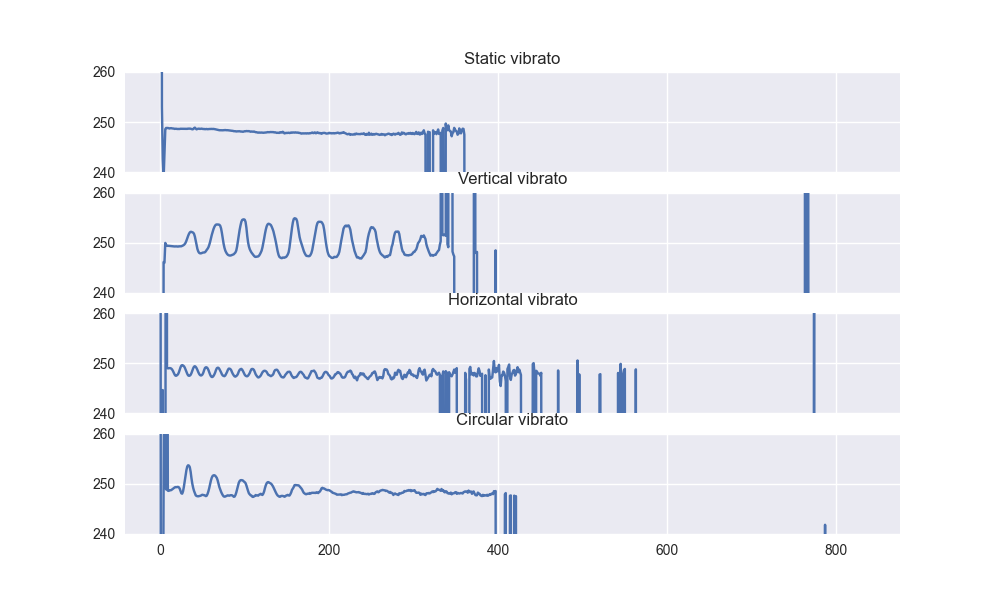
\includegraphics[width=1\columnwidth]{imgs/vibrato-comparison.png}
	\caption{Comparison of the spectrograms of different kinds of vibrato.}
	\label{fig:vibrato-spectrograms}
\end{figure}


\subsection{Machine learning}
A machine learning model will be trained to classify the kind of vibrato from the sensor data in the 4 classes: no vibrato, vertical vibrato, horizontal vibrato or circular vibrato. A regression model will be trained to infer the descriptors corresponding to hand movements.

\subsubsection{Vibrato type classification}

Sensors --> Vibrato class (static, vertical, horizontal, circular)
Sensors+Audio --> Vibrato class (static, vertical, horizontal, circular)


\subsubsection{Spectral centroid regression}
Sequence modeling 

Sensors --> Regression of harmonics and amplitude of the lowest five harmonics


\subsection{Interactive Music System}
Real-time mapping strategies for vibrato-aware guitar effects will be explored using a Pure Data interface and real-time hand motion capture and the trained models (eg. vibrato-dependent reverb, distortion, sustain, delay…).
\subsubsection{Vibrato-aware distortion}
\subsubsection{Vibrato transfer}
Vibrato on a synth note through physical modeling driven from sensor data.
PD vibrato


\section{Results}




\section{Conclusions}
Computational analysis of embodied technique allows to focus on nuance in the development of interactive music systems. However it is necessary to study the technique specifically taking into account the specificity of the instrument. 


%
% The following two commands are all you need in the
% initial runs of your .tex file to
% produce the bibliography for the citations in your paper.
\bibliographystyle{abbrv}

	\bibliography{nime-references} 

\end{document}
